% =============================================================================
\section{Architecture Overview}
% =============================================================================

\begin{frame}[plain]{MambaRefine-CD Architecture}
    \centering
    \vspace{-0.7em}
    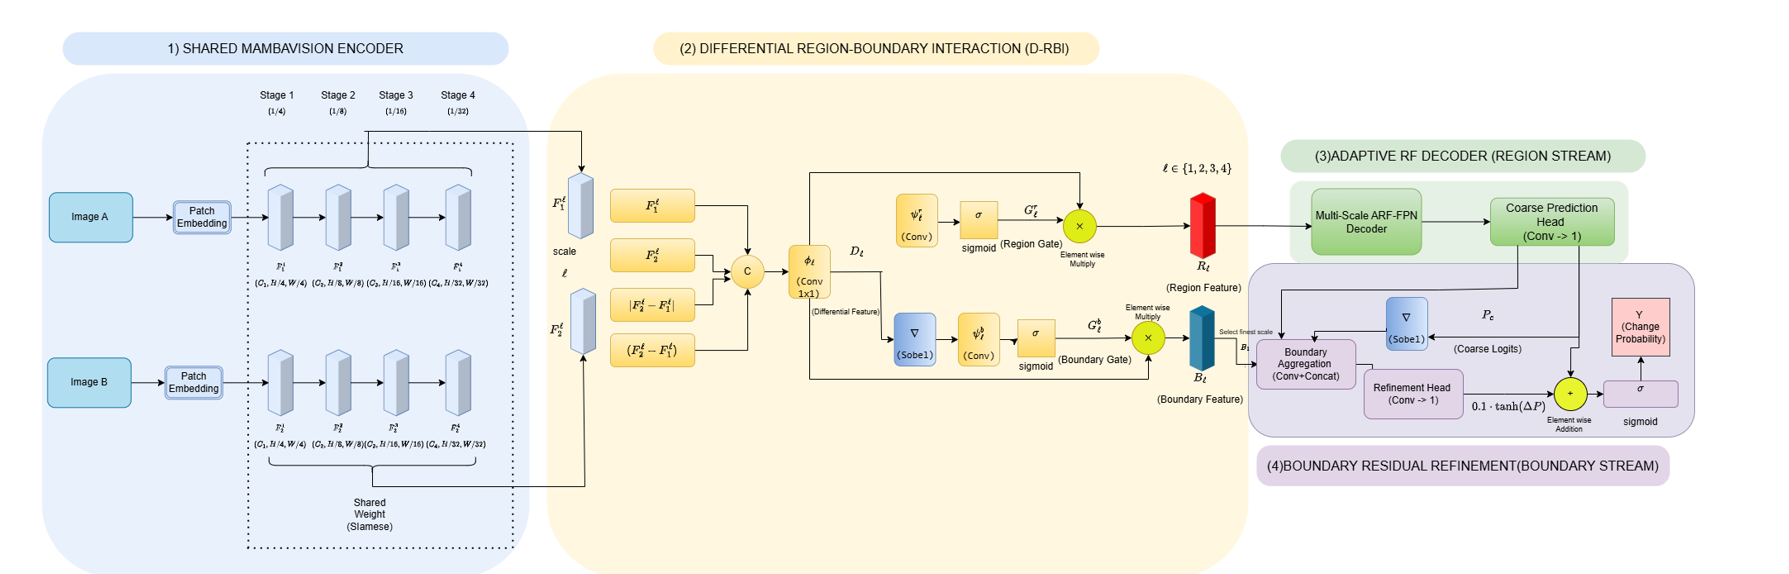
\includegraphics[width=0.99\textwidth,height=0.84\paperheight,keepaspectratio]{figures/architecture/architecture.png}
\end{frame}

\begin{frame}{High-Level Data Flow}
    \centering
    \begin{adjustbox}{max width=\textwidth,max height=0.34\textheight}
    \begin{tikzpicture}[node distance=6mm and 7mm]
        \node[tensor] (ia) {\(I_a\)};
        \node[tensor, below=5mm of ia] (ib) {\(I_b\)};
        \node[op, right=of $(ia)!0.5!(ib)$, text width=22mm] (enc) {Shared\\encoder};
        \node[op, right=of enc, text width=27mm] (td) {Temporal\\difference\\per scale};
        \node[op, right=of td, text width=24mm] (drbi) {D-RBI\\region +\\boundary};
        \node[fpn, right=of drbi, text width=24mm] (arf) {ARF-FPN\\coarse logits};
        \node[boundary, right=of arf, text width=24mm] (ref) {Boundary\\residual\\refinement};
        \node[tensor, right=of ref] (pf) {\(P_f\)};

        \draw[flowarrow] (ia) -| (enc);
        \draw[flowarrow] (ib) -| (enc);
        \draw[flowarrow] (enc) -- (td);
        \draw[flowarrow] (td) -- (drbi);
        \draw[flowarrow] (drbi) -- (arf);
        \draw[flowarrow] (arf) -- (ref);
        \draw[flowarrow] (ref) -- (pf);
    \end{tikzpicture}
    \end{adjustbox}

    \vspace{0.2em}
    \scriptsize
    \begin{align*}
    \{F_a^s\}_{s=0}^{3} &= E_\theta(I_a),\qquad
    \{F_b^s\}_{s=0}^{3}=E_\theta(I_b),\\
    \Delta^s &= F_b^s-F_a^s,\qquad
    D_{\mathrm{in}}^s=[|\Delta^s|;\Delta^s]\quad \text{for \texttt{abs\_signed}},\\
    (R^s,B^s) &= \operatorname{DRBI}_s(D_{\mathrm{in}}^s),\qquad
    P_c=\operatorname{ARFFPN}(\{R^s\}_{s=0}^{3}),\\
    P_f &= P_c+0.1\tanh(\Delta P_{\mathrm{raw}}).
    \end{align*}
\end{frame}

\begin{frame}{Shared MambaVision Encoder: Four Stages}
    \centering
    \vspace{-0.2em}
    \begin{adjustbox}{max width=\textwidth,max height=0.78\textheight}
    \begin{tikzpicture}[
        x=0.86mm,y=1mm,
        inputnode/.style={draw=black!50, rounded corners=2pt, thick, fill=black!3,
            minimum width=14mm, minimum height=28mm, align=center, inner sep=2pt, font=\scriptsize},
        stemblock/.style={draw=mvblue!70!black, thick, rounded corners=2pt,
            fill=mvblue!12, minimum width=7mm, minimum height=34mm,
            align=center, inner sep=1pt, font=\scriptsize},
        convblock/.style={draw=mvgreen!65!black, thick,
            fill=mvgreen!22, minimum width=9mm, minimum height=38mm,
            align=center, inner sep=1pt, font=\scriptsize},
        mixblock/.style={draw=mvgreen!65!black, thick,
            fill=mvgreen!18, minimum width=9mm, minimum height=38mm,
            align=center, inner sep=1pt, font=\scriptsize},
        mlpblock/.style={draw=mvorange!85!black, thick,
            fill=mvorange!15, minimum width=8mm, minimum height=38mm,
            align=center, inner sep=1pt, font=\scriptsize},
        downblock/.style={draw=mvorange!85!black, thick,
            fill=mvorange!8, minimum width=9mm, minimum height=38mm,
            align=center, inner sep=1pt, font=\scriptsize},
        featuretap/.style={-{Latex[length=2.2mm]}, very thick, draw=mvblue!75!black},
        stagefit/.style={draw=blue!75, very thick, dashed, rounded corners=5pt, inner sep=3.2mm},
        dimlabel/.style={font=\scriptsize, align=center, text=black!85},
        repeatlabel/.style={font=\scriptsize, text=mvblue, fill=white, inner sep=0.5pt}
    ]
        \node[inputnode] (img) at (0,0)
            {Input\\\(H\times W\times3\)};
        \node[stemblock] (stem) at (15,0) {\rotatebox{90}{Stem}};
        \node[convblock] (s1) at (28,0) {\rotatebox{90}{Conv Block}};
        \node[downblock] (d1) at (41,0) {\rotatebox{90}{Downsample}};
        \node[convblock] (s2) at (54,0) {\rotatebox{90}{Conv Block}};
        \node[downblock] (d2) at (67,0) {\rotatebox{90}{Downsample}};

        \node[mixblock] (mv3) at (82,0) {\rotatebox{90}{MambaVision Mixer}};
        \node[mlpblock] (mlp3a) at (92,0) {\rotatebox{90}{MLP}};
        \node[mixblock] (att3) at (104,0) {\rotatebox{90}{Self-Attn}};
        \node[mlpblock] (mlp3b) at (114,0) {\rotatebox{90}{MLP}};
        \node[downblock] (d3) at (128,0) {\rotatebox{90}{Downsample}};

        \node[mixblock] (mv4) at (143,0) {\rotatebox{90}{MambaVision Mixer}};
        \node[mlpblock] (mlp4a) at (153,0) {\rotatebox{90}{MLP}};
        \node[mixblock] (att4) at (165,0) {\rotatebox{90}{Self-Attn}};
        \node[mlpblock] (mlp4b) at (175,0) {\rotatebox{90}{MLP}};

        \begin{scope}[on background layer]
            \node[stagefit, fit=(mv3)(mlp3a)(att3)(mlp3b)] (g3) {};
            \node[stagefit, fit=(mv4)(mlp4a)(att4)(mlp4b)] (g4) {};
        \end{scope}

        \foreach \a/\b in {img/stem,stem/s1,s1/d1,d1/s2,s2/d2,d2/mv3,mv3/mlp3a,mlp3a/att3,att3/mlp3b,mlp3b/d3,d3/mv4,mv4/mlp4a,mlp4a/att4,att4/mlp4b}
            \draw[flowarrow] (\a) -- (\b);

        \node[repeatlabel, above=8mm of mv3] {\(\times\lceil N_3/2\rceil\)};
        \node[repeatlabel, above=8mm of att3] {\(\times\lfloor N_3/2\rfloor\)};
        \node[repeatlabel, above=8mm of mv4] {\(\times\lceil N_4/2\rceil\)};
        \node[repeatlabel, above=8mm of att4] {\(\times\lfloor N_4/2\rfloor\)};

        \draw[featuretap] (s1.south) -- ++(0,-6.2)
            node[below, font=\scriptsize, text=mvblue!75!black] {\(\mathbf{F^0}\)};
        \draw[featuretap] (s2.south) -- ++(0,-6.2)
            node[below, font=\scriptsize, text=mvblue!75!black] {\(\mathbf{F^1}\)};
        \draw[featuretap] (mlp3b.south) -- ++(0,-6.2)
            node[below, font=\scriptsize, text=mvblue!75!black] {\(\mathbf{F^2}\)};
        \draw[featuretap] (mlp4b.south) -- ++(0,-6.2)
            node[below, font=\scriptsize, text=mvblue!75!black] {\(\mathbf{F^3}\)};

        \node[dimlabel] at (28,-32)
            {\(\frac{H}{4}\times\frac{W}{4}\times C\)\\\textbf{Stage 1} \(\times N_1\)};
        \node[dimlabel] at (54,-32)
            {\(\frac{H}{8}\times\frac{W}{8}\times2C\)\\\textbf{Stage 2} \(\times N_2\)};
        \node[dimlabel] at (98,-32)
            {\(\frac{H}{16}\times\frac{W}{16}\times4C\)\\\textbf{Stage 3} \(\times N_3\)};
        \node[dimlabel] at (159,-32)
            {\(\frac{H}{32}\times\frac{W}{32}\times8C\)\\\textbf{Stage 4} \(\times N_4\)};
    \end{tikzpicture}
    \end{adjustbox}

    \vspace{0.2em}
    \scriptsize
    Encoder outputs are tapped after each stage:
    \(F^s\in\mathbb{R}^{B\times C2^s\times H/2^{s+2}\times W/2^{s+2}}\).
    For MambaVision-S: \(C=96\), \(N=(3,3,7,5)\).
\end{frame}

\begin{frame}{Encoder Block Equations}
    \small
    \begin{columns}[T,onlytextwidth]
        \begin{column}{0.43\textwidth}
            \centering
            \begin{adjustbox}{max width=\textwidth,max height=0.66\textheight}
            \begin{tikzpicture}[node distance=5.5mm]
                \node[tensor, text width=20mm] (x) {\(X\)};
                \node[op, below=of x, text width=24mm] (norm1) {Norm\\LN / BN};
                \node[op, below=of norm1, text width=28mm] (mix) {Token mixer\\Conv / Mamba\\/ Attention};
                \node[op, below=of mix, text width=24mm] (scale1) {\(\gamma_1\odot\)\\DropPath};
                \node[op, below=of scale1, circle, minimum size=7mm, inner sep=0pt] (add1) {\(+\)};
                \node[tensor, below=of add1, text width=20mm] (xp) {\(X'\)};
                \node[op, below=of xp, text width=24mm] (norm2) {Norm\\LN};
                \node[op, below=of norm2, text width=24mm] (mlp) {MLP};
                \node[op, below=of mlp, text width=24mm] (scale2) {\(\gamma_2\odot\)\\DropPath};
                \node[op, below=of scale2, circle, minimum size=7mm, inner sep=0pt] (add2) {\(+\)};
                \node[tensor, below=of add2, text width=24mm] (out) {\(X_{\mathrm{out}}\)};

                \draw[flowarrow] (x) -- (norm1);
                \draw[flowarrow] (norm1) -- (mix);
                \draw[flowarrow] (mix) -- (scale1);
                \draw[flowarrow] (scale1) -- (add1);
                \draw[flowarrow] (add1) -- (xp);
                \draw[flowarrow] (xp) -- (norm2);
                \draw[flowarrow] (norm2) -- (mlp);
                \draw[flowarrow] (mlp) -- (scale2);
                \draw[flowarrow] (scale2) -- (add2);
                \draw[flowarrow] (add2) -- (out);

                \draw[skiparrow] (x.east) -- ++(11mm,0) |- node[smallnote, pos=0.72, right] {skip} (add1.east);
                \draw[skiparrow] (xp.east) -- ++(11mm,0) |- node[smallnote, pos=0.72, right] {skip} (add2.east);
            \end{tikzpicture}
            \end{adjustbox}
        \end{column}
        \begin{column}{0.54\textwidth}
            \begin{align*}
            U &= \mathcal{M}(\operatorname{Norm}_1(X)),\\
            X' &= X+\operatorname{DropPath}(\gamma_1\odot U),\\
            V &= \operatorname{MLP}(\operatorname{Norm}_2(X')),\\
            X_{\mathrm{out}} &= X'+\operatorname{DropPath}(\gamma_2\odot V).
            \end{align*}
            \vspace{-0.2em}
            \scriptsize
            \[
            \mathcal{M}=
            \begin{cases}
            \text{convolutional residual stack}, & \text{stages 1--2},\\
            \text{MambaVision mixer or self-attention}, & \text{stages 3--4}.
            \end{cases}
            \]
            The block is pre-normalized and residual at both the token-mixing and MLP sublayers.
        \end{column}
    \end{columns}
\end{frame}

\begin{frame}{MambaVision Mixer Inside Stages 2--3}
    \centering
    \begin{adjustbox}{max width=\textwidth,max height=0.58\textheight}
    \begin{tikzpicture}[
        node distance=6mm and 8mm,
        branch/.style={draw=mvgreen!70!black, rounded corners=2pt, thick,
            fill=mvgreen!10, align=center, inner sep=3pt, minimum height=8mm,
            font=\scriptsize},
        scanop/.style={draw=mvblue!75!black, rounded corners=2pt, thick,
            fill=mvblue!8, align=center, inner sep=3pt, minimum height=8mm,
            font=\scriptsize},
        merge/.style={draw=mvorange!85!black, rounded corners=2pt, thick,
            fill=mvorange!10, align=center, inner sep=3pt, minimum height=8mm,
            font=\scriptsize}
    ]
        \node[tensor, text width=22mm] (x) at (0,0) {Window tokens\\\(B_w\times L\times C\)};
        \node[op, right=10mm of x, text width=20mm] (proj) {Linear\\in\_proj};
        \node[op, right=10mm of proj, text width=15mm] (split) {Split\\\([X_s,X_z]\)};

        \node[branch, above right=11mm and 10mm of split, text width=18mm] (xs) {SSM input\\\(X_s\)};
        \node[branch, right=8mm of xs, text width=24mm] (ssmconv) {same Conv1D\\+ SiLU\\\(U_s\)};
        \node[scanop, right=8mm of ssmconv, text width=24mm] (params) {\(x\_\)proj\\\(dt\_\)proj\\\(\Delta,B,C\)};
        \node[scanop, right=8mm of params, text width=23mm] (scan) {Selective\\Scan};
        \node[tensor, right=8mm of scan, text width=14mm] (ys) {\(Y_s\)};

        \node[branch, below right=11mm and 10mm of split, text width=18mm] (xz) {gate input\\\(X_z\)};
        \node[branch, right=8mm of xz, text width=24mm] (sym) {same Conv1D\\+ SiLU\\\(U_z\)};
        \node[tensor, text width=14mm] (uz) at (ys |- sym) {\(U_z\)};

        \node[merge, right=10mm of $(ys)!0.5!(uz)$, text width=18mm] (cat) {Concat\\\([Y_s;U_z]\)};
        \node[op, right=9mm of cat, text width=20mm] (outproj) {Linear\\out\_proj};
        \node[tensor, right=9mm of outproj, text width=18mm] (y) {Mixer\\output};

        \draw[flowarrow] (x) -- (proj);
        \draw[flowarrow] (proj) -- (split);
        \draw[flowarrow] (split.east) -- ++(5mm,0) |- node[smallnote, pos=0.25, right] {\(X_s\)} (xs.west);
        \draw[flowarrow] (split.east) -- ++(5mm,0) |- node[smallnote, pos=0.25, right] {\(X_z\)} (xz.west);
        \draw[flowarrow] (xs) -- (ssmconv);
        \draw[flowarrow] (ssmconv) -- (params);
        \draw[flowarrow] (params) -- (scan);
        \draw[flowarrow] (scan) -- (ys);
        \draw[flowarrow] (xz) -- (sym);
        \draw[flowarrow] (sym) -- (uz);
        \draw[flowarrow] (ys.east) -- ++(4mm,0) |- (cat.north);
        \draw[flowarrow] (uz.east) -- ++(4mm,0) |- (cat.south);
        \draw[flowarrow] (cat) -- (outproj);
        \draw[flowarrow] (outproj) -- (y);
    \end{tikzpicture}
    \end{adjustbox}

    \vspace{0.2em}
    \scriptsize
    \begin{align*}
    [X_s,X_z] &= \operatorname{split}(W_{\mathrm{in}}X),&
    U_s &= \operatorname{SiLU}(\operatorname{Conv1D}_{\mathrm{same}}(X_s)),\\
    U_z &= \operatorname{SiLU}(\operatorname{Conv1D}_{\mathrm{same}}(X_z)),&
    [\Delta_k,B_k,C_k] &= W_x U_{s,k},\\
    h_k &= \bar{A}_k h_{k-1}+\bar{B}_k U_{s,k},&
    Y &= W_{\mathrm{out}}[Y_s;U_z].
    \end{align*}
\end{frame}
